\documentclass[aspectratio=169]{beamer}
\usepackage[utf8]{inputenc}
%\usepackage[authordate,backend=biber,natbib]{biblatex-chicago}
%\usepackage{booktabs}
%\addbibresource{growthreferences.bib}

%\usepackage{utopia} %font utopia imported

\usetheme{Madrid}
\usecolortheme{beaver}

%------------------------------------------------------------
%This block of code defines the information to appear in the
%Title page
\title[Krugman (1979)] %optional
{Increasing Returns, Monopolistic Competition, and International Trade}

\subtitle{Paul Krugman, \emph{Journal of International Economics}, 1979}

\author [Hauk] % (optional)
{William~R.~Hauk,~Jr.} %\inst{1} %\and J.~Doe\inst{2}} 

\institute[UofSC] % (optional)
{
  %\inst{1}%
  Darla Moore School of Business\\
  University of South Carolina
  %\and
  %\inst{2}%
  %Faculty of Chemistry\\
  %Very Famous University
}

\date[ECON 860, Fall 2021] % (optional)
{ECON 860 -- International Trade Theory\\Fall 2021}

\logo{
\includegraphics[height=1cm]{UofSC_Monogram_Stack_CMYK_G.jpg}}

%End of title page configuration block

%---------------------------------------------------------

\AtBeginSection[]
{
  \begin{frame}
    \frametitle{Table of Contents}
    \tableofcontents[currentsection]
  \end{frame}
}

%------------------------------------------------------------

\begin{document}

%The next statement creates the title page.
\frame{\titlepage}

%-------------------------------------------------------------

\section{Introduction}

%-------------------------------------------------------------

\begin{frame}{A Bit of Intellectual History}

Adam Smith writes \emph{The Wealth of Nations} in 1776.  Points out three potential reasons that international trade might benefit a country:

\begin{enumerate}
    \item<1-> Specialization according to absolute advantage.  (``Uh, it’s more like comparative advantage." –David Ricardo)
    \item<2-> Increasing returns to scale from sales to larger markets.  (Pin factory example)
    \item<3-> Opportunity for consumers to consume a greater variety of goods.
\end{enumerate}
    
\end{frame}

%--------------------------------------------------------------

\begin{frame}{A Bit of Intellectual History}

\begin{itemize}
    \item<1-> For the next 200 or so years, nearly all analysis of trade focuses on the first reason.
    \item<2-> Some papers make use of increasing returns to scale: Ohlin (1933), Balassa (1967), and Kravis (1971), but increasing returns didn’t make it much into formal trade theory.  ``The main reason for this neglect seems to be that it has appeared difficult to deal with the implication for increasing returns for market structure."
    \item<3-> Paper develops a formal model in which trade is driven by economies of scale.  Market structure is similar to the Monopolistic Competition model of Dixit and Stiglitz (1977).
\end{itemize}
    
\end{frame}

%--------------------------------------------------------------

\section{Monopolistic Competition in a Closed Economy}

%--------------------------------------------------------------

\begin{frame}{Monopolistic Competition in a Closed Economy}

\begin{itemize}
    \item<1-> Assume an economy where labor is the only scarce factor of production.  Economy produces a large number of goods $ n $ indexed by $ i $.
    \item<2-> All consumers have the same utility function, where all goods enter symmetrically:
    \begin{equation}
        U = \sum_{i = 1}^{n}{v\left( c_{i} \right)} \text{ where } v' > 0 \text{ and } v'' < 0
        \label{eq:utilityfunction}
    \end{equation}
    \item<2-> Define a variable $ \varepsilon_i $ as:
    \begin{equation*}
        \varepsilon_{i} = -\frac{v'}{v''c_{i}}
    \end{equation*}
    (in equilibrium, this will be the elasticity of demand of good $ i $) and assume that $ \frac{\partial \varepsilon_{i}}{\partial c_{i}} < 0 $ (this is true for a linear demand function and anything ``less convex" than a CES demand curve).
\end{itemize}
    
\end{frame}

%--------------------------------------------------------------

\begin{frame}{Output}

\begin{itemize}
    \item<1-> All goods are produced using the same cost function.  The labor used in producing each good is a linear function of output:
    \begin{equation*}
        l_{i} = \alpha + \beta x_{i}
    \end{equation*}
    where $ l_{i} $ is the amount of labor used producing good $ i $, $ x_i $ is the output of good $ i $, and $ \alpha $ is a fixed cost.
    \item<2-> Note that this function implies that there are positive fixed costs, constant marginal costs, and therefore decreasing average costs. (i.e. increasing returns to scale)
\end{itemize}
    
\end{frame}

%--------------------------------------------------------------

\begin{frame}{Employment and Consumption}

\begin{itemize}
    \item<1-> Production of the good must equal the sum of individual consumptions of the good, so:
    \begin{equation}
        x_{i} = L c_{i}
        \label{eq:consumptionproduction}
    \end{equation}
    where $ L $ is the size of the labor force.
    \item<2-> Finally, assume full employment in equilibrium, so that:
    \begin{equation*}
        L = \sum_{i = 1}^{n}l_{i} = \sum_{i = 1}^{n}\left[ \alpha + \beta x_{i} \right]
    \end{equation*}
\end{itemize}
    
\end{frame}

%---------------------------------------------------------------

\begin{frame}{Autarky Equilibrium}

In order to characterize the autarky equilibrium, we need to determine three variables:

\begin{enumerate}
    \item The price of each good relative to the wage rate, $ \frac{p_{i}}{w}$.
    \item The output of each good, $ x_{i} $.
    \item The number of goods produced, $ n $.
\end{enumerate}

Due to the symmetry of the utility and cost functions, we can assume that $ p_{i} = p $ and $ x_{i} = x $ for all $ i $.
    
\end{frame}

%----------------------------------------------------------------

\begin{frame}{Equilibrium Solution Steps}

Three steps to finding an equilibrium:

\begin{enumerate}
    \item<1-> First, analyze the demand curve facing an individual firm.
    \item<2-> Second, derive the pricing policy of firms and relate profitability to output.
    \item<3-> Third, look at profitability and entry to determine the number of firms.  
\end{enumerate}
    
\end{frame}

%-----------------------------------------------------------------

\subsection{Demand Curves Facing Firms}

%------------------------------------------------------------------

\begin{frame}{Demand Curves Facing Firms}

\begin{itemize}
    \item<1-> The first-order conditions that follow from the utility function have the form:
    \begin{equation}
        v'\left( c_{i} \right) = \lambda p_{i}
        \label{eq:FOC}
    \end{equation}
    \item<2-> If we substitute (\ref{eq:consumptionproduction}) into equation (\ref{eq:FOC}), we can derive an expression for the demand curve facing and individual firm:
    \begin{equation*}
        p_{i} = \lambda^{-1} v'\left( \frac{x_{i}}{L} \right)
    \end{equation*}
    \item<3-> If the number of goods produced is relatively large, then each firm’s pricing policy should have a negligible effect on the marginal utility of income, so we can treat $ \lambda $ as fixed.  We can then show that the elasticity of demand facing firm $ i $ is $ \varepsilon_{i} = -\frac{v'}{v'' c_{i}} $.
\end{itemize}
    
\end{frame}

%------------------------------------------------------------------

\subsection{Firm Pricing Policy}

%------------------------------------------------------------------

\begin{frame}{Firm Pricing Policy}

\begin{itemize}
    \item<1-> We assume that each firm is relatively small to the overall economy, and can ignore the effects of its pricing decision on other firms.  The $ i $th firm maximizes the profit function:
    \begin{equation}
        \Pi_{i} = p_{i} x_{i} - \left( \alpha + \beta x_{i} \right)
        \label{eq:profitfunction}
    \end{equation}
    \item<2-> The profit maximizing price depends on the marginal cost and on the elasticity of demand:
    \begin{equation*}
        p_{i} = \frac{\varepsilon_{i}}{\varepsilon_{i} - 1} \beta w
    \end{equation*}
    which we can rewrite as:
    \begin{equation}
        \frac{p_{i}}{w} = \beta \frac{\varepsilon_{i}}{\varepsilon_{i} - 1}
        \label{eq:optimalprice}
    \end{equation}
\end{itemize}
    
\end{frame}

%------------------------------------------------------------------

\subsection{Profitability and the Number of Firms}

%------------------------------------------------------------------

\begin{frame}{Profitability and the Number of Firms \#1}

Profits are driven to zero by the free entry and exit of firms.  Figure 1 shows the total cost ($ TC $) while $ OR $ and $ OR^{1} $ represent revenue functions.  The firm maximizes profits when the revenue function has the same slope as the cost function (i.e. $ MC = MR $).
\begin{figure}
     \centering
     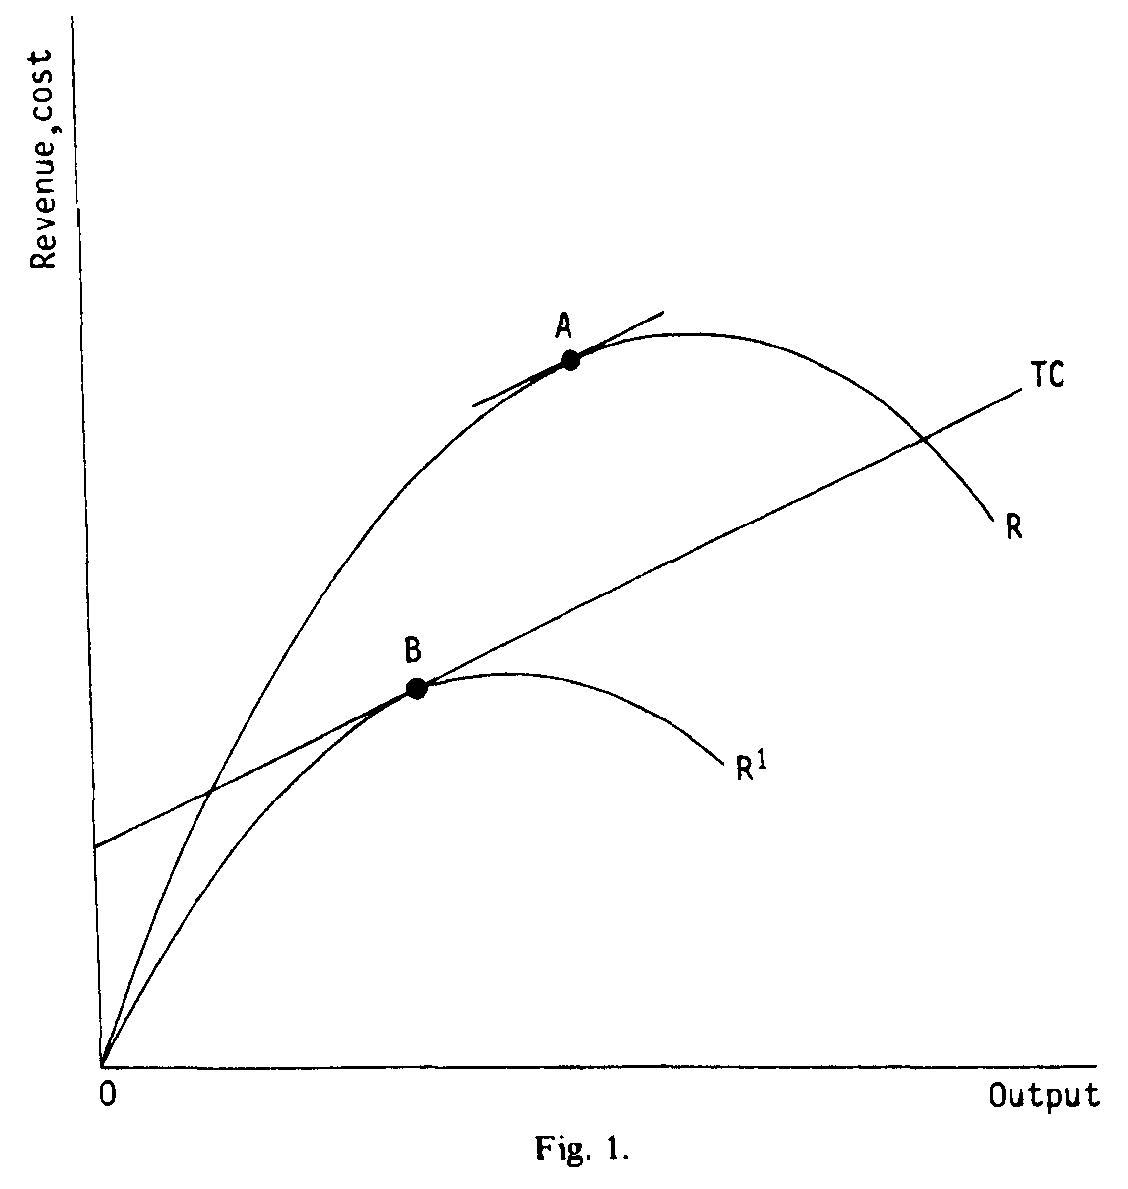
\includegraphics[scale=0.45]{KrugmanFig1.jpg}
     \label{fig:figure1}
\end{figure}
    
\end{frame}

%------------------------------------------------------------------

\begin{frame}{Profitability and the Number of Firms \#2}

Figure 2 shows the relationship between $ c $ and $ \frac{p}{w} $, because the elasticity of demand falls as $ c $ increases, curve $ PP $ is sloping upwards hyperbolically from $ \beta $.
\begin{figure}
     \centering
     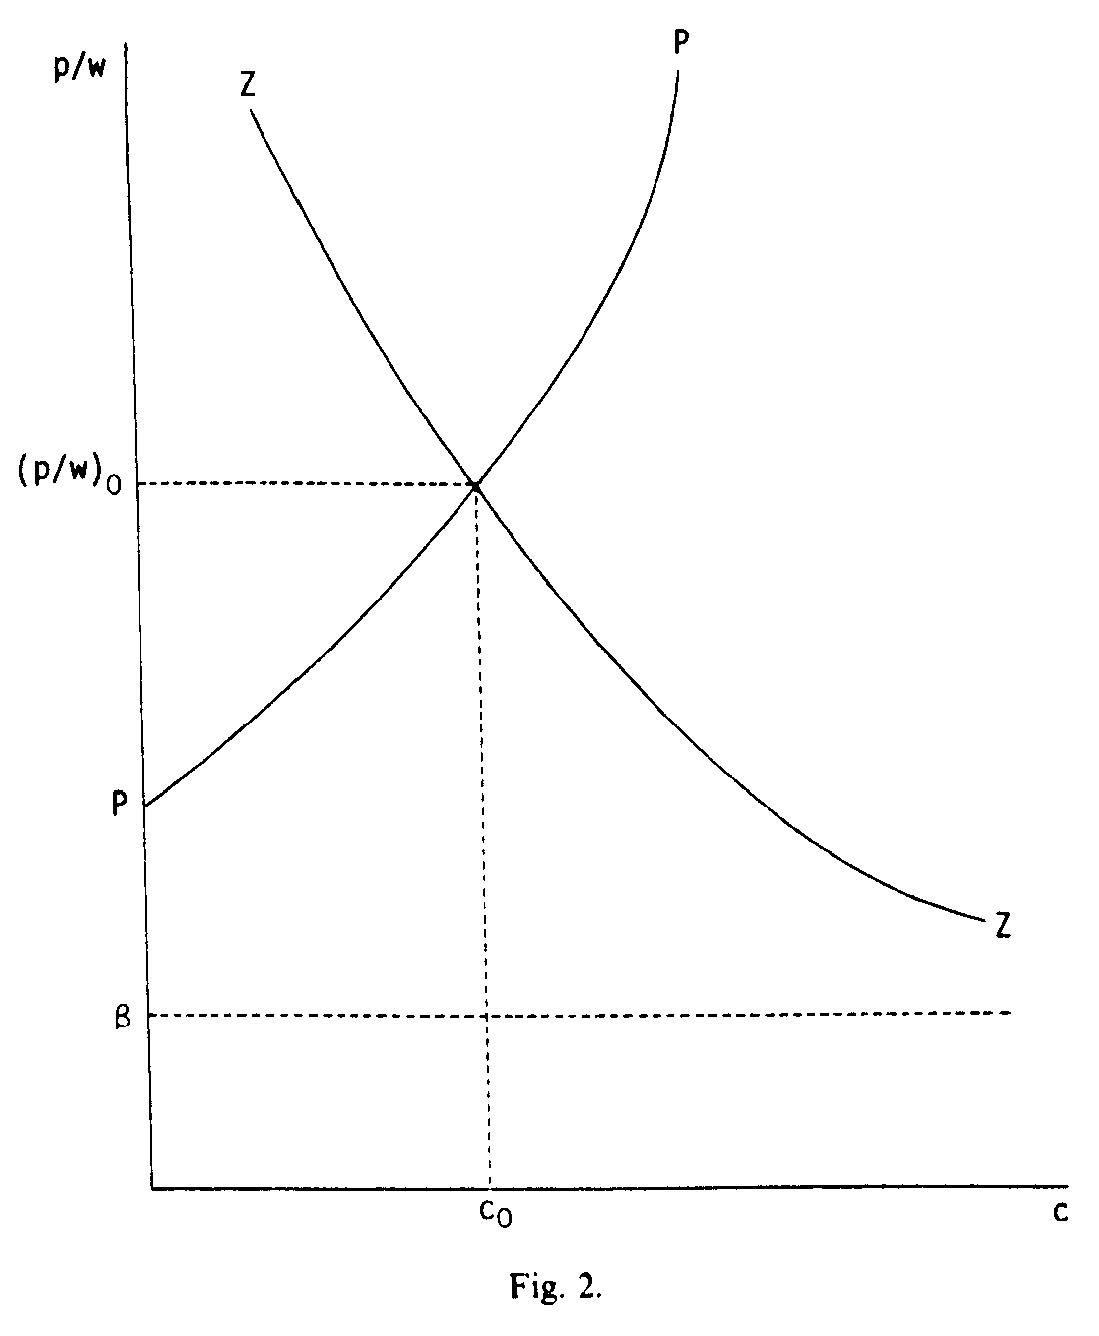
\includegraphics[scale=0.13]{KrugmanFig2.jpg}
     \label{fig:figure2}
\end{figure}
    
\end{frame}

%------------------------------------------------------------------

\begin{frame}{Profitability and the Number of Firms \#3}

\begin{itemize}
    \item<1-> To find the zero profit condition, note that we can rewrite equation (\ref{eq:profitfunction}) as:
    \begin{equation}
        \begin{split}
            0 &= px - \left( \alpha + \beta x \right) w \\
            \frac{p}{w} &= \beta + \frac{\alpha}{Lc}
        \end{split}
        \label{eq:zeroprofitcondition}
    \end{equation}
    where the 2nd line uses the fact that $ x = Lc$.
    \item<2-> The zero-profit condition converges hyperbolically towards $ \beta $ and is represented by curve $ ZZ $ in Figure 2.
    \item<3-> We can find the equilibrium level of  $ \frac{p}{w} $ and $ c $ by looking at the intersection of $ PP $ and $ ZZ $.  Because $ x = Lc $, finding $ c $ gives us the equilibrium output for each firm (which by assumption is symmetric across firms).  Furthermore, we can determine the number of goods produced using our full employment condition:
    \begin{equation}
        n = \frac{L}{\alpha + \beta x}
        \label{eq:numberofgoods}
    \end{equation}
\end{itemize}
    
\end{frame}

%------------------------------------------------------------------

\section{Growth, Trade, and Factor Mobility}

%------------------------------------------------------------------

\begin{frame}{Market Size Matters}

This section considers three ways in which the size of the market might increase:
\begin{enumerate}
    \item Growth in the labor force.
    \item International trade.
    \item International migration.
\end{enumerate}
    
\end{frame}

%-------------------------------------------------------------------

\subsection{Effects of Labor Force Growth}

%-------------------------------------------------------------------

\begin{frame}{Labor Force Growth \#1}

An increase in the labor force $ L $ would not affect the $ PP $ curve according to equation (\ref{eq:optimalprice}).  However, according to equation (\ref{eq:zeroprofitcondition}), the $ ZZ $ curve would shift down and to the left as depicted in Figure 3.
\begin{figure}
     \centering
     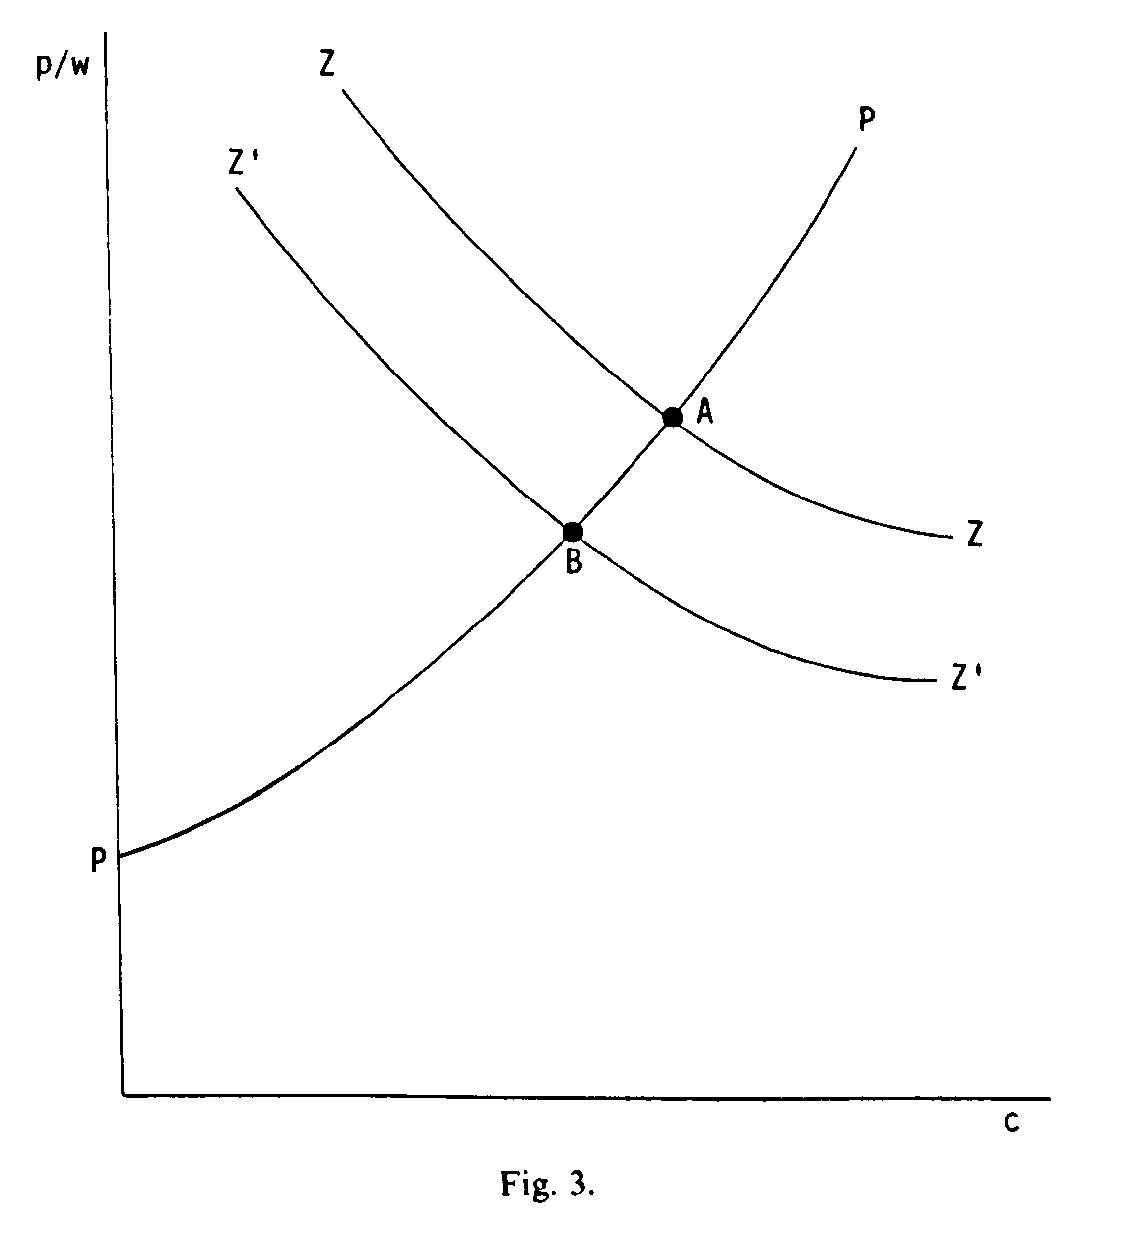
\includegraphics[scale=0.125]{KrugmanFig3.jpg}
     \label{fig:figure3}
\end{figure}
    
\end{frame}

%-------------------------------------------------------------------

\begin{frame}{Labor Force Growth \#2}

\begin{itemize}
    \item<1-> According to Figure 3,  $ \frac{p}{w} $ would fall and the per-capita consumption of each good $ c $ would decrease.
    \item<2-> However, the output of each good $ x $ would increase, as we can see by rearranging equation (\ref{eq:zeroprofitcondition}):
    \begin{equation*}
        x = \frac{\alpha}{\frac{p}{w} - \beta}
    \end{equation*}
    that is, if $ \frac{p}{w} $ falls, then $ x $ should rise.
    \item<3-> Also, the number of varieties of goods produced will increase, which we can see from equation (\ref{eq:numberofgoods}):
    \begin{equation*}
        n = \frac{L}{\alpha + \beta Lc} = \frac{1}{\frac{\alpha}{L} + \beta c}
    \end{equation*}
    a rise in $ L $ and a fall in $ c $ will lead to an increase in $ n $.
\end{itemize}
    
\end{frame}

%--------------------------------------------------------------------

\begin{frame}{Labor Force Growth \#3}

\begin{itemize}
    \item<1-> Note – this result does make use of the assumption that $ \varepsilon_{i} $ falls as $ c_{i} $ increases.  This assumption will become an issue in the subsequent literature.
    \item<2-> The welfare implications of this increase in the labor force are positive:  the real wage $ \frac{w}{p} $ has increased and the number of varieties of goods available has increased.
\end{itemize}
    
\end{frame}

%--------------------------------------------------------------------

\subsection{Effects of Trade}

%--------------------------------------------------------------------

\begin{frame}{Effects of Trade \#1}

This section of the paper is a thought experiment:
\begin{itemize}
    \item<1-> Suppose that there are two countries that are identical in terms of tastes and production technologies.
    \item<2-> They would have no differences in opportunity costs, no differences in comparative advantage, and therefore, no reason to trade under classical models.
    \item<3-> Assume that these two countries open up to trade with each other and there are no transportation costs.
\end{itemize}
    
\end{frame}

%--------------------------------------------------------------------

\begin{frame}{Effects of Trade \#2}

\begin{itemize}
    \item<1-> The number of goods produced in each country will be proportional to the labor forces:
    \begin{equation*}
        \begin{split}
            n &= \frac{L}{\alpha + \beta x} \\
            n^{*} &= \frac{L^{*}}{\alpha + \beta x}
        \end{split}
    \end{equation*}
    \item<2-> As the market size increases, the scale of production $ x $ increases.
    \item<3-> The number of varieties produced in each country falls, even though the total varieties of goods available to consumers rises.  That is, if  $ N^{A} $ is the number of varieties produced in each country under autarky, and $ N^{T} $ is the number of varieties available to consumers with trade, then $ N^{A} < N^{T} < 2N^{A} $.
    \item<4-> Some firms will exit the market after the trade opening, but that the remaining firms will be larger.
\end{itemize}
    
\end{frame}

%--------------------------------------------------------------------

\subsection{Effects of Factor Mobility}

%--------------------------------------------------------------------

\begin{frame}{Factor Mobility}

\begin{itemize}
    \item<1-> Mundell (1957) notes that factor movements may effective act as a substitute for trade and vice versa.  This model has similar results.
    \item<2-> If there are impediments to trade (e.g. tariffs or transportation costs) there will be an incentive for workers to move to the country or region that has the largest population (higher real wages, greater variety of goods).
    \item<3-> This result can help to explain agglomeration effects.
\end{itemize}
    
\end{frame}

%--------------------------------------------------------------------

\section{Empirical Studies}

\subsection{Broda and Weinstein (2006)}

%--------------------------------------------------------------------

\begin{frame}{Broda and Weinstein (2006); Gains from Variety}

\begin{itemize}
    \item<1-> One of the gains from trade in this model is from the increase in varieties available to consumers.
    \item<2-> The magnitude of this gain is difficult to measure because we don’t know what the willingness to pay of a consumer is until a good is available.
    \item<3-> This is, in principle, similar to the new goods problem from measuring inflation.
    \item<4-> Broda and Weinstein (2006) attempt to quantify the gains to U.S. consumers from greater import variety.
\end{itemize}
    
\end{frame}

%--------------------------------------------------------------------

\begin{frame}{Sato-Vartia Price Index}

Sato (1976) and Vartia (1976) demonstrate that, if we start from a Constant Elasticity of Substitution (CES) utility function, we can construct an ``exact” price index based on the minimum expenditure necessary to get a unit of utility as a function of prices if there is a constant set of goods $ I $:
\begin{equation*}
    \frac{e\left( p_{t}, I \right)}{e\left( p_{t-1}, I \right)} = P_{SV}\left( p_{t-1}, p_{t}, c_{t-1}, c_{t} \right) = \prod_{i \in I}{\left( \frac{p_{i,t}}{p_{i,t-1}} \right)^{w_{i}\left( I \right)}}
\end{equation*}
where the weights $ w_{i}\left( I \right) $ are constructed from expenditure shares $ s_{i,t}\left( I \right) = \frac{p_{i,t} c_{i,t}}{\sum_{i \in I}{p_{i,t} c_{i,t}}} $ and are given by:
\begin{equation*}
    w_{i}\left( I \right) =  \frac{\left( \frac{s_{i,t}\left( I \right) - s_{i,t-1}\left( I \right)}{\ln{s_{i,t}\left( I \right)} - \ln{s_{i,t-1}\left( I \right)}} \right)}{\sum_{i \in I}{\left( \frac{s_{i,t}\left( I \right) - s_{i,t-1}\left( I \right)}{\ln{s_{i,t}\left( I \right)} - \ln{s_{i,t-1}\left( I \right)}} \right)}}
\end{equation*}
    
\end{frame}

%--------------------------------------------------------------------

\begin{frame}{Feenstra Price Index and New Goods}

The Sato-Vartia index works well if the set of goods isn’t changing, but that’s the issue here.  Feenstra (1994) shows that the SV index can be modified in the following way: for $ i \in I \subseteq I_{t-1} \cap I_{t} $, for $ \sigma > 1 $:
\begin{equation*}
    \frac{e\left( p_{t}, I \right)}{e\left( p_{t-1}, I \right)} = P_{SV}\left( p_{t-1}, p_{t}, c_{t-1}, c_{t} \right)\left( \frac{\lambda_{t}\left( I \right)}{\lambda_{t-1}\left( I \right)} \right)^{1 / \left( 1 - \sigma \right)}
\end{equation*}
where the $ \lambda $ values are determined by the fraction of expenditures on goods common to both periods using the formula:
\begin{equation*}
    \lambda_{t}\left( I \right) = \frac{\sum_{i \in I}p_{i,t} c_{i,t}}{\sum_{i \in I_{t}}p_{i,t} c_{i,t}}
\end{equation*}
    
\end{frame}

%--------------------------------------------------------------------

\begin{frame}{Broda and Weinstein Estimates}

\begin{itemize}
    \item<1-> Broda and Weinstein note that, especially during the period after the fall of the Soviet Union, the U.S. imported goods from a lot of countries that it didn’t before.
    \item<2-> For data from 1989-2001, they define a variety of a good as a 10-digit HS import from a particular country, and from 1972-1988 as a 7-digit TSUSA import from a particular country.
    \item<3-> They use these data to estimate $ \sigma $ for different industries and calculate $ \left( \frac{\lambda_{t}\left( I \right)}{\lambda_{t-1}\left( I \right)} \right)^{1 / \left( 1 - \sigma \right)} $ from 1972-2001.
    \item<4-> They find that the gains in variety of goods alone is worth about $ 2.6\% $ of U.S. GDP.
\end{itemize}
    
\end{frame}

%--------------------------------------------------------------------

\subsection{Trefler (2004)}

%--------------------------------------------------------------------

\begin{frame}{CUSFTA of 1989}

\begin{itemize}
    \item<1-> In 1989, Canada signed a free-trade agreement with the U.S. (a few years later, Mexico was added to it, and it became NAFTA).
    \item<2-> The agreement was sold, in part, on the idea that scale economies would especially beneficial for Canada.
    \item<3-> This prediction has not been borne out very well empirically.  Head and Ries (1999) look at Canadian plant-level data, find that tariff reductions in the U.S. increased plant scale in Canada by $ 10\% $, but this was offset by tariff reductions in Canada reducing plant scale by about $ 8.5\% $. 
\end{itemize}
    
\end{frame}

%--------------------------------------------------------------------

\begin{frame}{Trefler (2004) Study}

\begin{itemize}
    \item<1-> Trefler (2004) finds that, after the CUSFTA, the plants most exposed to U.S. imports saw the highest gains in productivity – about $ 14\% $.  However, he does not find statistically significant scale effects.
    \item<2-> The effect on productivity comes predominantly from selection effects – the least productive firms are the most likely to exit the market, whereas the most productive firms remain.
    \item<3-> The Krugman (1979) model assumes perfect symmetry across firms, so asymmetry in firms dropping out of market is not part of its predictions.  Melitz (2003) model that we’ll discuss next week will introduce heterogeneous firms.
\end{itemize}
    
\end{frame}

%--------------------------------------------------------------------

\section{Conclusions}

%--------------------------------------------------------------------

\begin{frame}{Conclusions}

\begin{itemize}
    \item<1-> Krugman introduces a few big things into the international trade literature: increasing returns to scale, gains from variety, and intra-industry trade.
    \item<2-> However, some predictions rely on a scale effect from larger markets.  This prediction seems questionable empirically – we need to add more to the model to understand gains from trade and variety.
\end{itemize}
    
\end{frame}

%--------------------------------------------------------------------

\end{document}